%----------------------------------------------------------------------------------------
%	PACKETS AND CONFIGURATION
%----------------------------------------------------------------------------------------

\documentclass[12pt, a4paper]{article}

\usepackage{times} % Times New Roman font
\usepackage{graphicx} % 'graphics' package interface
\usepackage{geometry} % Edit document margins
\usepackage{hyperref} % Table of contents hyperlinks
\usepackage{tcolorbox} % Colored boxes for code
\usepackage[font=small, labelfont=bf]{caption} % Image caption font
\usepackage{longtable} % Build long tables

% HELPER PACKAGES (REMOVE IN FINAL) %
\usepackage{blindtext} % Lorem Ipsum
\usepackage{todonotes} % TODOs as useful reminders
\setlength{\marginparwidth}{2cm} % Otherwise todonotes gets angry at me lol
\setuptodonotes{fancyline, color=green!40, shadow} % TODOs options
% HELPER PACKAGES (REMOVE IN FINAL) %

\graphicspath{ {./res/} } % Path to graphics
\hypersetup{    % ToC Hyperlink setup
    colorlinks,
    citecolor=blue,
    filecolor=blue,
    linkcolor=blue,
    urlcolor=blue
}

%----------------------------------------------------------------------------------------
%	DOCUMENT
%----------------------------------------------------------------------------------------

\begin{document}

\newgeometry{top=7cm, bottom=2cm} % Setting the margins for the title

% Title
\begin{titlepage}
    \centering
    {\Huge\bfseries Pandemic Information System Model\par} % Project title
    \vspace{1.5cm}
    {\scshape\large Systems and Methods for Big and Unstructured Data \par} % Course
    \vspace{0.5cm}
    {\scshape\large Prof. Marco Brambilla \par} % Professor
    \vspace{1cm}
    {\scshape\large % Description
        Second delivery \par 
        MongoDB Project \par 
    }
    \vspace{0.5cm}
    {\slshape\large December 2021 \par} % Date
    \vspace{1cm}
    \linespread{0.8} % Authors interline
    {\large\itshape % Authors
        Avci Oguzhan - \texttt{10557284}\\
        Gentile Nicole - \texttt{10594355}\\
        Rigamonti Davide - \texttt{10629791}\\
        Singh Raul - \texttt{10623232}\\
        Tagliaferri Mattia - \texttt{10572418}
    }
    \vfill
    \begin{figure}[b]
        
\includegraphics[scale=0.6]{polimi.png} % Polimi logo
        \centering
    \end{figure}

    \pagenumbering{gobble} % Remove page number

\end{titlepage}

\newgeometry{bottom=3cm} % Reset the margins
\pagenumbering{arabic} % Reset the page number

\clearpage

% INDEX
{
    \hypersetup{hidelinks}
    \tableofcontents
}

% LIST OF TODOs (REMOVE IN FINAL)
\listoftodos

\clearpage

% INTRODUCTION
\section{Introduction}

\subsection{Problem Specification}

The idea of the project is that of building a dataset containing information about 
\emph{"green"} certifications and people/organizations acquiring and releasing them. \\ 
A certificate is released whenever a person takes a vaccination shot, takes a test to 
check if they are infected with Covid-19 of if they recovered from Covid-19. \\
All certificates contain information about the person 
involved, the organization issuing the certificate and information about the vaccine or 
the test. \\
The purpose of this project is to build a system that allows to check the validity of 
these certificates according to the latest government rules.

\subsection{Hypoteses}

\begin{itemize}

    \item Vaccines and tests
    \begin{itemize}
        \item[] We assumed that vaccines and tests can be used 
            as soon as they are produced without accounting for delivery time.
        \item[] Similarly to what happens in reality, we assumed that there is one
            certification for each test/vaccine, so that a person can have different 
            certifications associated but not all of them may be valid at a given time.
        \item[] We also assumed that the minimum time elapsed between two doses
            for the same person is at least one day in order to have a better
            distribution of vaccinations inside the generated dataset;
            furthermore, all doses must be of the same vaccine brand and a
            single person can have up to 3 vaccine doses. 
        \item[] Given the previous assumptions we don't consider the test 
            results to have any relevance besides for negative tests
            generating a certification that is valid for a certain amount of 
            time.        
	\item[] Moreover, we assumed positive tests are not stored in this database, since
	certificates are meaningful only for vaccinated or healed people.
        \item[] Vaccines are produced from 01/01/2021 to 26/11/2021 with a
            number ranging from 0 to 2 lots per day, adding up to a total
            of 330 lots numbered from \emph{1} to \emph{330}.
        \item[] Tests are performed from 01/01/2021 to 26/11/20 21 and 
            their lots are numbered from \emph{1200} to \emph{1600}.
        \item[] The validity check for green passes is performed by the application 
            (more on this can be found in the Application section of this document).
    \end{itemize}

    \item Other entities
    \begin{itemize}
        \item[] The SSN field for people is considered to be a unique
            identifier for the single individual.
        \item[] Names for regular people, doctors, cities and authorized bodies 
            have no relevance and were chosen randomly, therefore information 
            such as phone numbers for people and coordinates for authorized 
            bodies aren't designed to be consistent among the dataset.
        \item[] All authorized bodies can release all kinds of certificates.
        \item[] People were born between years 1941 and 2011, therefore their 
            age ranges roughly from \emph{10 y.} to \emph{80 y.} considering 
            2021 to be current year.
    \end{itemize}

\end{itemize}
  
\clearpage

% DATABASE
\section{Database}

\subsection{Document Diagram}
\begin{figure}[h]
    \makebox[\textwidth][c]{ % Box to properly center the image
        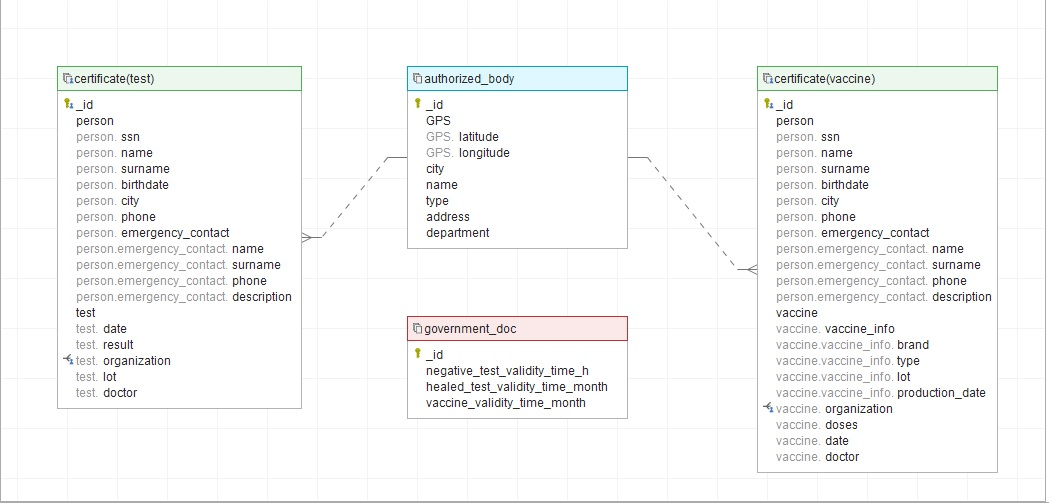
\includegraphics[scale=0.65]{doc_diagram.png} % ER diagram
    }
    \caption*{The diagram represents the first phase of the database design.} % Caption
\end{figure}

\noindent 
Since in this project we used a documental database, we decided to use a document diagram.
The elements in the diagram are:
\begin{itemize}
    \item \texttt{Authorized Body}: it contains information about any organization that can release vaccines or tests.
    \item \texttt{Government doc}: it represents the government rules about the duration of the various types of certificates. The validity is expressed in hours for the negative tests, while it is expressed in months for vaccines and tests done after healing from Covid-19.
    \item \texttt{Certificate}: there are two types of certificates: one for tests and one for vaccines. Test certificates include information about the result of the test, while vaccine certification include brand, type, production date of the vaccine and the number of the dose. Both contain information about the owner, including its emergency contact, the lot of test/vaccine, the organization that released it, the date it was made, the doctor who was attending.

\end{itemize}
\subsection{Dataset description}

We represented a population of about 200 people taking a total of 330 vaccinations
(190 first doses, 120 second doses and 20 third doses) and 300 tests inside
a total of 270 authorized bodies (130 hospitals, 80 pharmacies and 60 
specialized centers). \\
Certifications are characterized by information about the related person
(SSN, name, surname, birthdate, city, phone number and an emergency contact
including the name, surname, phone number and description for a person to 
contact in case of emergency) and the vaccination (date, organization, doctor 
and information about the vaccine such as brand, type, lot and production 
date) or the test (lot, result, date, organization and doctor). \\
Authorized bodies are characterized by: GPS coordinates (latitude and longitude), city,
name, type (pharmacy, hospital or specialized centers), address and department 
(only for hospitals). \\
There is also a document containing informations about the latest government rules
on the time validity of tests and vaccines certifications; we assumed test validity is 
24 hours (whereas in case a negative test implies that the person has healed, its 
duration is extended to 6 months), while vaccinations validity is 9 months. \\
The complete script used for the creation of the dataset, together with a 
database dump will be provided alongside this document.

% VIEWS
\subsection{Views}
Views are used to make queries easier to be executed.

\subsubsection{Certificates with datetimes}
This view is used to convert all dates contained in certificates to datetime format. 
Moreover, we also add a field representing the age of the person.

\begin{tcolorbox}[fontupper=\scriptsize]
    \begin{verbatim}
db.createView(
"certificate_datetimes", 
"certificate", 
[
	{"$addFields":{
	        "vaccine.date": {
	        "$dateFromString": {
	          "dateString": "$vaccine.date"
	        }
	      },	       
	       "test.date": {
	        "$dateFromString": {
	          "dateString": "$test.date"
	        }
	      },      
	       "person.birthdate": {
	        "$dateFromString": {
	          "dateString": "$person.birthdate"
	        }
	      }
	}},
	{"$addFields":{
	  "person.age": {
	        "$subtract": [{ $year: new Date() },
	        { $year: "$person.birthdate" }]
	      }
	}}
])
    \end{verbatim}
\end{tcolorbox}

\subsubsection{Join bewteen certificates and authorized bodies}
This view is used to retrieve the information about the authorized bodies issuing 
vaccinations or tests.
\begin{tcolorbox}[fontupper=\scriptsize]
    \begin{verbatim}
db.createView(
"certificate_authorizedBodies", 
"certificate", 
[
	{ "$addFields":{
	  "vaccine.organization": {
	    "$toObjectId": "$vaccine.organization"}
	    ,  
	    "test.organization": {
	    "$toObjectId": "$test.organization"}
	  }
	},
	{"$lookup": {
	    "from": "authorized_bodies",
	    "localField": "vaccine.organization",
	    "foreignField": "_id",
	    "as": "vaccine.organization"
	  }
	},
	{"$lookup": {
	    "from": "authorized_bodies",
	    "localField": "test.organization",
	    "foreignField": "_id",
	    "as": "test.organization"
	  }
	}
])
    \end{verbatim}
\end{tcolorbox}

%QUERIES
\subsection{Queries}

\subsubsection{Check validity by SSN}
\begin{tcolorbox}[fontupper=\scriptsize]
    \begin{verbatim}
db.certificate.find( {  "person.ssn": ssn,
  "vaccine.doses": { "$gt": n_dose }}
)
    \end{verbatim}
\end{tcolorbox}

\noindent % Removes indentation after box
Checks if a specific person has a newer vaccine dose than the specified one. \\
The query is used to invalidate old vaccination certificates. \\
It takes the following parameters:
\begin{itemize}
    \item \texttt{ssn} \emph{(string)}: social security number of the person;
    \item \texttt{n\_dose} \emph{(int)}: number of the dose.
\end{itemize}
		
\subsubsection{Defective Lot}
\begin{tcolorbox}[fontupper=\scriptsize]
    \begin{verbatim}
db.certificate.find(  {"vaccine.vaccine_info.lot": lot},
				{"person.ssn":1,
				"person.name":1,
				"person.surname":1,
				"person.phone":1})
    \end{verbatim}
\end{tcolorbox}

\noindent % Removes indentation after box
Returns SSN, name, surname and phone number of people vaccinated with the specified 
defective vaccine lot. \\
It takes the following parameters:
\begin{itemize}
    \item \texttt{lot} \emph{(int)}: number of the defective lot.
\end{itemize}

\subsubsection{Find Certificate by Id}
\begin{tcolorbox}[fontupper=\scriptsize]
    \begin{verbatim}
db.certificate.find(
{"_id": ObjectId(id)
 })
    \end{verbatim}
\end{tcolorbox}

\noindent % Removes indentation after box
Returns the certificate with a given id. The retrieved document is later used to check 
its validity according to the date, the government rules and, in case of vaccine, the 
presence of newer vaccinations. \\
It takes the following parameters:
\begin{itemize}
    \item \texttt{id} \emph{(string)}: id of the certificate.
\end{itemize}

\subsubsection{Percentage of fully vaccinated people by age groups}
\begin{tcolorbox}[fontupper=\scriptsize]
    \begin{verbatim}
// total number of people
var personNumber = db.certificate.distinct("person.ssn").length;

// divide people into groups and calcultate the percentage of second doses 
// for each group 
db.certificate_datetimes.aggregate(
      {$match: {"vaccine.doses": 2}},
      {$group: {
        _id: {
            $concat: [
              {$cond: [ {$and: [ 
                            {$lt: ["$person.age", 20]} ]}, "Under 20", ""]},
              {$cond: [ {$and: [ {$gte: ["$person.age", 20]}, 
                            {$lt: ["$person.age", 40]} ]}, "20 - 40", ""]},
              {$cond: [ {$and: [ {$gte: ["$person.age", 40]}, 
                            {$lt: ["$person.age", 50]} ]}, "40 - 50", ""]},
              {$cond: [ {$and: [ {$gte: ["$person.age", 50]}, 
                            {$lt: ["$person.age", 60]} ]}, "50 - 60", ""]},
              {$cond: [ {$and: [ {$gte: ["$person.age", 60]}, 
                            {$lt: ["$person.age", 70]} ]}, "60 - 70", ""]},
              {$cond: [ {$gte: ["$person.age", 70]}, "Over 70", ""]},
            ]
        },
        count: {$sum: 1},
      }},
      {$project: {
        count: 1,
        percentage: {$multiply:[{$divide: ["$count", personNumber]}, 100]}
      }},
      {$sort: {_id: 1}}
 )
    \end{verbatim}
\end{tcolorbox}
\noindent 
Returns the percentage of fully vaccinated people (i.e. the ones having at least the 
second dose of vaccine) divided by age groups.

\subsubsection{Percentage of boosters by age groups}
\begin{tcolorbox}[fontupper=\scriptsize]
    \begin{verbatim}
// find the percentage of boosters (3rd dose) for each age group
var personNumber = db.certificate.distinct("person.ssn").length;
db.certificate_datetimes.aggregate(
      {$match: {"vaccine.doses": 3}},
      {$group: {
        _id: {
          $concat: [
              {$cond: [ {$and: [ {$gte: ["$person.age", 10]},
                            {$lt: ["$person.age", 20]} ]}, "Under 20", ""]},
              {$cond: [ {$and: [ {$gte: ["$person.age", 20]}, 
                            {$lt: ["$person.age", 40]} ]}, "20 - 40", ""]},
              {$cond: [ {$and: [ {$gte: ["$person.age", 40]}, 
                            {$lt: ["$person.age", 50]} ]}, "40 - 50", ""]},
              {$cond: [ {$and: [ {$gte: ["$person.age", 50]}, 
                            {$lt: ["$person.age", 60]} ]}, "50 - 60", ""]},
              {$cond: [ {$and: [ {$gte: ["$person.age", 60]}, 
                            {$lt: ["$person.age", 70]} ]}, "60 - 70", ""]},
              {$cond: [ {$gte: ["$person.age", 70]}, "Over 70", ""]},
            ]
        },
        count: {$sum: 1},
      }},
      {$project: {
        count: 1,
        percentage: {$multiply:[{$divide: ["$count", personNumber]}, 100]}
      }},
      {$sort: {_id: 1}}
 )
    \end{verbatim}
\end{tcolorbox}
\noindent 
Returns the percentage of people having the 3rd dose for each age group.

\subsubsection{Percentage of vaccinated by age groups}
\begin{tcolorbox}[fontupper=\scriptsize]
    \begin{verbatim}
var personNumber = db.certificate.distinct("person.ssn").length;

db.certificate_datetimes.aggregate(
      {$match: {"vaccine.doses": 1}},
      {$group: {
        _id: {
          $concat: [
              {$cond: [ {$and: [ {$gte: ["$person.age", 10]},
                            {$lt: ["$person.age", 20]} ]}, "Under 20", ""]},
              {$cond: [ {$and: [ {$gte: ["$person.age", 20]}, 
                            {$lt: ["$person.age", 40]} ]}, "20 - 40", ""]},
              {$cond: [ {$and: [ {$gte: ["$person.age", 40]}, 
                            {$lt: ["$person.age", 50]} ]}, "40 - 50", ""]},
              {$cond: [ {$and: [ {$gte: ["$person.age", 50]}, 
                            {$lt: ["$person.age", 60]} ]}, "50 - 60", ""]},
              {$cond: [ {$and: [ {$gte: ["$person.age", 60]}, 
                            {$lt: ["$person.age", 70]} ]}, "60 - 70", ""]},
              {$cond: [ {$gte: ["$person.age", 70]}, "Over 70", ""]},
            ]
        },
        count: {$sum: 1},
      }},
      {$project: {
        count: 1,
        percentage: {$multiply:[{$divide: ["$count", personNumber]}, 100]}
      }},
      {$sort: {_id: 1}}
 )
    \end{verbatim}
\end{tcolorbox}
\noindent 
Returns the percentage of people who got the 1st dose for each age group.

\subsubsection{Number of people with only the first dose}
\begin{tcolorbox}[fontupper=\scriptsize]
    \begin{verbatim}
// find the ssn of people having the first dose
var first_dose = db.certificate.find({"vaccine.doses": 1}).count()

// count number of people having the second dose
var second_dose = db.certificate.find( { "vaccine.doses":2 } ).count()

first_dose - second_dose
    \end{verbatim}
\end{tcolorbox}

\noindent 
Returns how many people did the first dose but not the second.

\subsubsection{Percentage of vaccinated people}
\begin{tcolorbox}[fontupper=\scriptsize]
    \begin{verbatim}
// find total number of vaccinated people 
// (i.e. the ones having at least the first dose)
var total_vaccinated = db.certificate.find({"vaccine.doses": 1}).count()

// find total number of people
var total_people = db.runCommand(
   {
      distinct: "certificate",
      key: "person.ssn",
   }
).values.length

// calculate the percentage
total_vaccinated/total_people * 100
    \end{verbatim}
\end{tcolorbox}

\noindent
Returns the percentage of vaccinated people over the total number of people.

\subsubsection{Number of tests per organization}
\begin{tcolorbox}[fontupper=\scriptsize]
    \begin{verbatim}
db.certificate_authorizedBodies.aggregate( [  
{ $sortByCount: "$test.organization.name" } ] )
    \end{verbatim}
\end{tcolorbox}

\noindent
Returns the number of tests made by each organization.

\subsubsection{Number of vaccines per organization}
\begin{tcolorbox}[fontupper=\scriptsize]
    \begin{verbatim}
db.certificate_authorizedBodies.aggregate( [  
{ $sortByCount: "$vaccines.organization.name" } ] )
    \end{verbatim}
\end{tcolorbox}

\noindent
Returns the number of vaccines made by each organization.

\subsubsection{Number of vaccines per brand}
\begin{tcolorbox}[fontupper=\scriptsize]
    \begin{verbatim}
db.certificate.aggregate( [ { $sortByCount: "$vaccine.vaccine_info.brand" } ] )
    \end{verbatim}
\end{tcolorbox}

\noindent
Returns the number of vaccines made for each brand:
\begin{itemize}
    \item \emph{'Moderna'},
    \item \emph{'Johnson \& Johnson'}
    \item \emph{'Pfizer-BioNTech'}
    \item \emph{'AstraZeneca'}
\end{itemize}

\subsubsection{Number of vaccines per type}
\begin{tcolorbox}[fontupper=\scriptsize]
    \begin{verbatim}
db.certificate.aggregate( [ { $sortByCount: "$vaccine.vaccine_info.type" } ] )
    \end{verbatim}
\end{tcolorbox}

\noindent
Returns the number of vaccines made for each type ('Genetic' or 'Viral vector').

\subsection{Commands}

\subsubsection{Add new vaccine} 
\begin{tcolorbox}[fontupper=\scriptsize]
    \begin{verbatim}
db.certificate.insertOne(
{ 
    "person": {
    "ssn": ssn,
    "name": name,
    "surname": surname,
    "birthdate": birthdate,
    "city": city,
    "phone": phone,
    "emergency_contact": {
        "name": e_name,
        "surname": e_surname,
        "phone": e_phone,
        "description": description
        }
    },
    "vaccine": {
        "vaccine_info": {
            "brand": brand,
            "type": type,
            "lot": lot,
            "production_date": prod_date
        },
    "organization": id_org,
    "doses": doses,
    "date": vaccine_date,
    "doctor": doctor
    }
});
    \end{verbatim}
\end{tcolorbox}

\noindent
Inserts a new vaccine in the database. All dates are expressed as strings
in "YYYY-MM-DD" format. \\
It takes the following parameters:
\begin{itemize}
    \item \texttt{ssn} \emph{(string)}: social security number of the person;
    \item \texttt{name} \emph{(string)}: name of the person;
    \item \texttt{surname} \emph{(string)}: surname of the person;
    \item \texttt{birthdate} \emph{(string)}: birthdate of the person;
    \item \texttt{city} \emph{(city)}: city where the person lives;
    \item \texttt{phone} \emph{(string)}: phone number of the person;
    \item \texttt{e\_name} \emph{(string)}: name of the emergency contact;
    \item \texttt{e\_surname} \emph{(string)}: surname of the emergency contact;
    \item \texttt{e\_phone} \emph{(string)}: phone of the emergency contact;
    \item \texttt{description} \emph{(string)}: description of the emergency contact;
    \item \texttt{brand} \emph{(string)}:brand of the vaccine;
    \item \texttt{type} \emph{(string)}: type of the vaccine;
    \item \texttt{lot} \emph{(int)}: lot of the vaccine;
    \item \texttt{prod\_date} \emph{(string)}: production date of the vaccine;
    \item \texttt{id\_org} \emph{(string)}: id of the organization releasing the vaccine;
    \item \texttt{doses} \emph{(int)}: number of the vaccine dose;
    \item \texttt{vaccine\_date} \emph{(string)}: date of the vaccine;
    \item \texttt{doctor} \emph{(string)}: name of the doctor attending the vaccination.
 \end{itemize}

\subsubsection{Delete old tests}
\begin{tcolorbox}[fontupper=\scriptsize]
    \begin{verbatim}
db.certificate_datetimes.find({ 
  "test.date": {"$lte": new Date(new Date().setMonth(new Date().getMonth()-3))}
}).forEach(function(doc) {
    db.certificate.deleteMany({ "_id": doc._id });
  });
      \end{verbatim}
\end{tcolorbox}

\noindent
Delete all tests older than 3 months.

\subsubsection{Update emergency contact}
\begin{tcolorbox}[fontupper=\scriptsize]
    \begin{verbatim}
db.certificate.updateMany(
	{"person.ssn": ssn},
	{"$set" : {
		"person.emergency_contact.name": name,
		"person.emergency_contact.surname": surname,
		"person.emergency_contact.phone": phone,
		"person.emergency_contact.description": description	
		}
	})
      \end{verbatim}
\end{tcolorbox}

\noindent
Updates the emergency contact of a certain person. \\
It takes the following parameters:
\begin{itemize}
    \item \texttt{ssn} \emph{(string)}: social security number of the person;
    \item \texttt{name} \emph{(string)}: name of the emergency contact;
    \item \texttt{surname} \emph{(string)}: surname of the emergency contact;
    \item \texttt{phone} \emph{(string)}: phone of the emergency contact;
    \item \texttt{description} \emph{(string)}: description of the emergency contact;
 \end{itemize}

\subsubsection{Update government rules} 
\begin{tcolorbox}[fontupper=\scriptsize]
    \begin{verbatim}
db.government_rules.updateOne(
          {},
          {"$set" : { 
                    "negative_test_validity_time_h": negative_test_time,
                    "healed_test_validity_time_month": healed_test_time, 
                    "vaccine_validity_time_month": vaccine_time
          }})
      \end{verbatim}
\end{tcolorbox}

\noindent
Updates the government rules about the validity of tests and vaccines. \\
It takes the following parameters:
\begin{itemize}
    \item \texttt{test\_time} \emph{(int)}: hours for which a negative test is valid;
    \item \texttt{vaccine\_months} \emph{(int)}: months for which a vaccine is valid;
    \item \texttt{healed\_test\_time} \emph{(int)}: months for which a test obtained after 
        healing from Covid-19 is valid.
 \end{itemize}

\clearpage

% APPLICATION
\section{Application}

\subsection{Description}

The app is split into 3 tabs: 
\begin{itemize}
    \item The first tab contains a panel where you can request the generation of a
        QR code for a certificate given the SSN of a person. \\ 
        You can choose to generate a certificate related to the vaccine doses' 
        certificates, the most recent negative test or the most recent healed test. \\ 
        After generating it, a \emph{.png} file containing the QR code is saved on your 
        working directory where the JAR has been launched. 
    \item The second tab contains a panel where you can choose an image containing a QR 
        code and checks if the associated certificate is valid or not. \\
        A certificate is judged as valid if the corresponding certificate is found inside
        the database (retrieved using its id encoded in \emph{base64}) and matches the 
        validity conditions given for its certificate type. 
If the id of a certificate is not found in the database, then the certificate is not valid.
If it is found and it is a vaccine, we check there are no newer vaccines made after it, otherwise it is not valid; then we check that the date matches the validity conditions given by the government. If the certificate is a test, we simply check its date according to government rules.
    \item (Please note that this works only if you run the application on Windows) The 
        third tab contains a panel that integrates a webcam component capable of 
        scanning the QR code and checks its validity.
\end{itemize}

\subsection{User Guide}

The app is written in Java, therefore it requires Java 11 or newer versions in order to 
run properly. \\
There are two JAR files, one with the webcam version (intended to be run on Windows), 
and the other one without the webcam. 
It will work only if the cluster on MongoDB is created with a username called 
\emph{‘admin’} and password \emph{‘psw’}, while database name must be \emph{‘project2’}. \\
The collections' names must be: 
\begin{itemize}
    \item ‘authorized\_body‘;
    \item ‘certificate‘;
    \item ‘government\_doc‘.
\end{itemize}


\clearpage % Here otherwise the screenshots go in strange places

\subsection{Screenshots}

\begin{figure}[h]
    \centering
    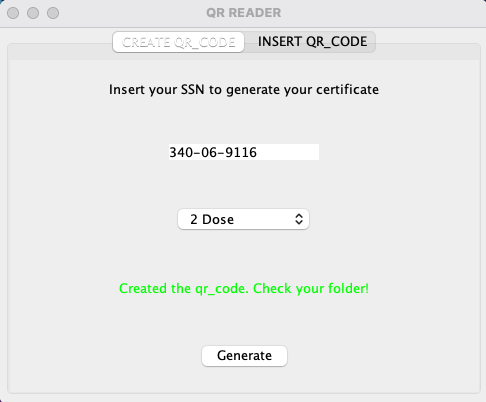
\includegraphics[width=.6\linewidth]{app_1.png}
    \caption*{Generation of a QR code.} % Caption
\end{figure}
\vspace{2cm}
\begin{figure}[h]
    \centering
    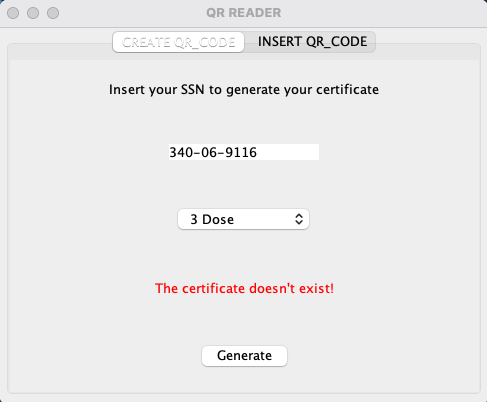
\includegraphics[width=.6\linewidth]{app_2.png}
    \caption*{Trying to generate a QR code for a non-existing certificate.} % Caption
\end{figure}
\begin{figure}[h]
    \centering
    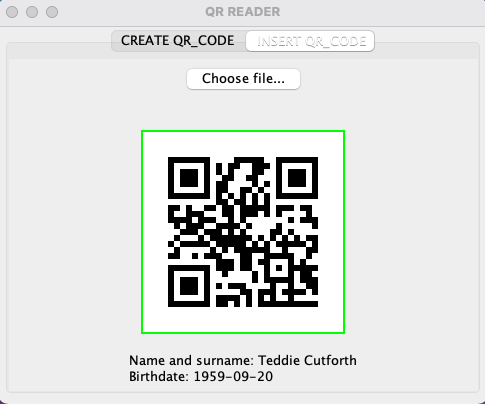
\includegraphics[width=.6\linewidth]{app_3.png}
    \caption*{Scan of a valid QR code.} % Caption
\end{figure}
\begin{figure}[h]
    \centering
    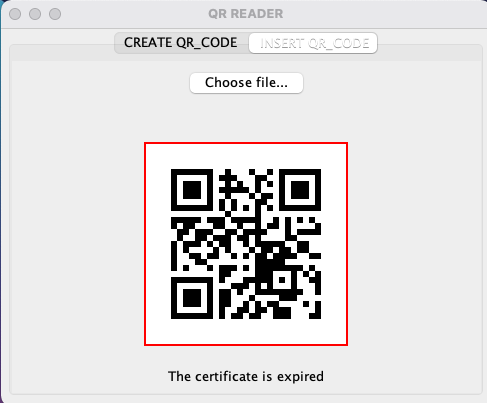
\includegraphics[width=.6\linewidth]{app_4.png}
    \caption*{Scan of an invalid Qr code.} % Caption
\end{figure}
\begin{figure}[h]
    \centering
    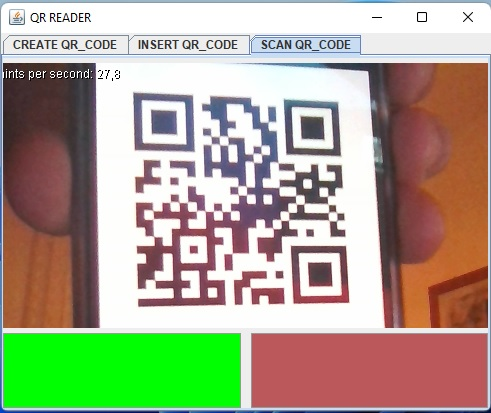
\includegraphics[width=.6\linewidth]{app_5.png}
    \caption*{Scan of a valid QR code via webcam.} % Caption
\end{figure}
\begin{figure}[h]
    \centering
    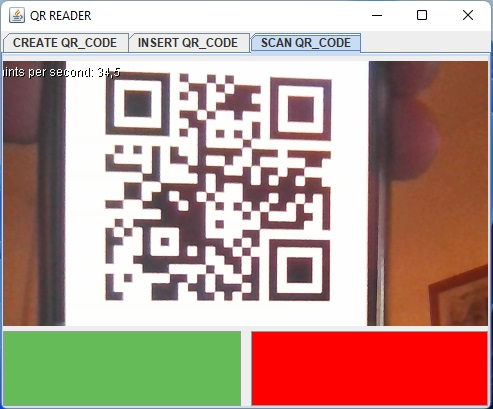
\includegraphics[width=.6\linewidth]{app_6.png}
    \caption*{Scan of an invalid Qr code via webcam.} % Caption
\end{figure}

\clearpage 

% REFERENCES AND SOURCES
\section{References and sources}

In order to develop these project, the following tools were used:

\begin{itemize}
    \item MongoDB and the MongoDB Compass to build and navigate the database 
        and write queries;
    \item \LaTeX~to write the report;
    \item Github as a versioning and collaboration mean;
    \item Java, JavaFX, Scene builder, MongoDB Driver and the ZXing library to build 
        the application;
    \item \url{https://www.Mockaroo.com} 
        to generate realistic data for people, authorized bodies and 
        certifications;
    \item \href{https://data.gov.sg/dataset/listing-of-licensed-pharmacies}{link}
        to the resource used for the pharmacy population;
    \item \href{https://corgis-edu.github.io/corgis/csv/hospitals/}{link}
        to the resource used for the hospital population.
\end{itemize}

\clearpage

\end{document}